
\documentclass[12pt,PhD]{muthesis}

\usepackage{verbatim}
\usepackage{graphicx}
\usepackage{url} % typeset URL's reasonably
\usepackage{listings}
\usepackage{phdthesis}
\usepackage{rotating}
\usepackage{subfig}
\usepackage{psfrag}
\usepackage{varioref}
\usepackage{appendix}
\usepackage{booktabs}
\usepackage{nomencl}

\makenomenclature

\begin{document}

\title{Amino acid biosynthetic cost in gene expression and evolution}
\author{Michael D. Barton}
\principaladviser{Casey M. Bergman}

\beforeabstract

\printnomenclature[1.5cm]

\prefacesection{Abstract}
Abstract text

\afterabstract

\prefacesection{Acknowledgements}
I would like to thank...
\afterpreface

\chapter{Introduction}
\input{1_introduction}
\chapter{Estimating amino acid cost and gene fitness using flux balance analysis}
\section*{Summary}

Using genome scale models to estimate cost has precedent in the estimates of oxygen related shadow prices in the work of Varma \emph{et al.} \cite{varma1993}. In chapter I have illustrated how similar methods can be used to estimate amino acid costs and how these costs show a high degree of similarity with previous measures of energetic cost, or atomic content. Furthermore new measures of amino acid cost have been estimated taking into consideration the estimated quantity of the amino acid present in biomass.

\clearpage

\section{Introduction}

\subsection{Understanding biological systems}

Early enzymology predicted rate limiting steps in biological pathways. The slowest step in the pathway will limit the rate at which the pathway acts. If the rate of the slowest step is increased, then intuition suggests that the rate of the entire pathway will increase proportionally. When attempting to modulate the flux through the tryptophan biosynthetic pathway in yeast Niederberger \emph{et. al} \cite{niederberger1992} found that individual up or down regulation of specific enzymes had little overall effect on tryptophan biosynthesis. Instead the rate of the biosynthetic pathway could instead be increased by increasing the quantity of five related enzymes in tandem. This research is an example control in a biological system being distributed over the system as a whole rather than focused at individual points.

The theory of metabolic control analysis \cite{fell} states that there are no rate limiting steps in biological systems, but instead that each part of the systems shares a measure of control, with some parts having more control than others. The control an enzyme has on the rest of the system can determined by measuring the effect of its up or down modulation on the reaction in question. For example in metabolic control analysis the control of enzyme X on reaction Y can be described mathematically as follows.

\begin{equation}\label{fcc}
C_{X}^{Y} = \frac{dX}{X}\div\frac{dY}{Y}
\end{equation}

The function $\frac{dX}{X}$ represents the effect of a small change in the reaction flux through reaction X, given the original flux. The function $\div\frac{dY}{Y}$ represents the proportional change in Y resulting from the change in X. Metabolic control analysis defines the ratio of these two functions as the flux control coefficient of reaction X on reaction Y using the nomenclature $C_{X}^{Y}$. Larger values of $C_{X}^{Y}$ indicate that reaction X has a high degree of control on reaction Y. Smaller values indicate that reaction Y experiences only small change in flux in response to changes in X.

Determining a numeric value for the relationships between reactions in a metabolic network allows properties of biological systems to be explored. For example Westerhoff \emph{et al.} \cite{hierarchical_control} predicted with an \emph{in silico} model of yeast glycolysis \cite{teusink} which reaction were controlled via changes in enzyme quantity and which were controlled by increasing in metabolite concentrations.

WAS TEUSINK MODEL USED?
INSERT EXAMPLES OF MCA USE

Other aspects of metabolic control theory is the prediction of metabolite control coefficients, whereby metabolite concentrations will have a degree of control on the rate of reactions.

INSERT EXAMPLES OF MCC use.

\subsection{Stoichiometric approaches}

\emph{In silico} kinetic models require specific information about enzyme activity for each reaction. In the case of an enzyme that follows simple Michalis-Menten kinetics parameters such as Km and Vmax are sufficient. To model more complex enzymatic reactions requires larger numbers of parameter sets which require more experimental effort to derive. This means that kinetic model of biological processes are often small with a limited number of reaction sets, due to the difficulty in finding sufficient enzymatic data for the reactions in the system. Stoichiometric models do not require kinetic data but instead only the connectivity between reactions, the participating metabolites and the \emph{in vivo} direction of the reaction.

Requiring less data for construction, stoichiometric models are much larger than kinetic models. Genome scale stoichiometric models can be constructed from the genome sequence of the organism through identifying the presence of enzymes, and connecting the encoded reactions based on metabolic maps. An iterative process of simulation can identify possible missing reactions required for viable growth \cite{genome_model_construction}. The growth rate of the model is simulated through of linear optimisation problem to maximise a given objective reaction such as the production of biomass defined in the combination of internal reaction and the available nutrients.

Genome scale models can be used to predict which \emph{in silico} single \cite{single_knockout} or double \cite{double_knockout} gene deletions lead to an \emph{in vivo} lethal or sick phenotype. Further \emph{in silico} analysis predicts that additional genes making a significant contribution to growth could be identified through multiple gene knockout \cite{deutscher2008}.

INSERT FURTHER FBA EXAMPLES HERE

Similar to the calculation of metabolite control coefficients described in the previous section, stoichiometric models can be used to calculate the shadow price of a molecule. In economics the shadow price, for example of a sold product, represents the effect in changes of prices on the market. Varma \emph{et al.} \cite{varma1993} transfered the use of shadow prices to biology and used this in the estimation of the shadow price of oxygen on \emph{E. coli} energy metabolism. Through simulating a decrease in the availability of oxygen the researchers identified how the shadow prices of the redox carriers changed with the availability of oxygen. The research showed that with decreasing availability of oxygen, the shadow price of oxygen use rises, this leads to a decrease in the shadow price of ethanol for energy production decreases as it becomes instead used to eliminate redox and secreted.

\subsection{Estimating the cost of amino acids}

\subsubsection{Energetic cost}

The article by Varma \emph{et al.} highlights how systems biology models can be used to estimate the importance of a set of metabolites to cell growth. Related to this is the question of how much it costs the cell to synthesise and use amino acids. Craig \& Weber \cite{craig1998} estimated the cost of the twenty amino acids as the sum of how many high energy phosphate bonds (e.g. ATP) and reducing molecules (e.g. NADPH) are diverted from the available energy pool in the synthesis of each amino acid from glucose. The aim of deriving these costs was to estimate the importance of amino acid cost the evolution of a set of \emph{E. coli} proteins.

Akashi \& Gojobori \cite{akashi2002} explored a similar approach calculating cost on a range different energy sources to estimate the importance of amino acid cost in predicted \emph{E. coli} and \emph{B. subtilis} gene expression. Heizer \emph{et al.} \cite{heizer} expanded this estimating amino acid cost for inorganic sources in their analysis of the genomes of four prokaryotic species including photoautotrophs. These estimates of cost are based on the curation of the metabolic network to account for the expenditure of high energy molecules during synthesis. Seligmann argued \cite{seligmann2004} that the cost of amino acid biosynthesis must take into account more than just the energy required for synthesis. Seligmann used molecular weight as a proxy amino acid cost arguing that this may take into account investments in synthesising larger more complex amino acids. Using molecular weight also has the advantage where the metabolic network in not required to curate the number of high energy molecules used during synthesis.

DOUBLE CHECK AKASHI PAPER
HOW IS WAGNER'S COST DIFFERENT

\subsubsection{Atomic content}

Amino acid synthesis will require energy to power each step in the metabolic network, in addition to the energetic cost the molecules part of the amino acid structure may also be considered a cost of synthesis. Mazel \& Marliere \cite{mazel1989} showed that \emph{Calothrix} proteins expressed in sulphur limiting conditions are depleted for sulphur containing cysteine and methionine amino acids. This work indicating the atomic content of an amino acid should also be taken into consideration when attempting to define a measure of cost. Work by both Baudoin-Cornu \emph{et al.} \cite{baudoin2001} and Bragg \emph{et al.}	\cite{bragg2006} used atomic content as a measure of amino acid cost when examining protein content.

\subsection{Summary of results}

The results presented in this chapter are split into two sections. The first describes an approach to estimating amino acid cost focusing on the \emph{S. cerevisiae} genome scale metabolic model. The approach used to estimate amino acid cost is similar to that described by Varma \emph{et al.} in their estimation of the shadow prices in \emph{E.coli} energy metabolism. The estimated costs are compared to the other estimates of amino acid cost that appear in the literature described above.

The second part of results section describes an experimental approach to estimate the cost of a gene. This is again in \emph{S. cerevisiae} using the genome scale metabolic model. This approach performs a type of robustness analysis on the gene encoded metabolic function. This analysis produces a robustness distribution describing how increasing and decreasing metabolic rate for an function affect the \emph{in silico} model fitness.

\clearpage

\section{Results}

The biomass equation in a flux balance analysis model describes the estimated requirements and stoichiometry of metabolites required growth. In the biomass reaction in the \emph{S. cerevisiae} model, the requirements include fats such as triglyceride and ergosterol, sugars such as glucose and mannose, as well as smaller metabolites sulphate and water. The stoichiometry of the biomass equation is derived from the dry weight biomass of the \emph{S. cerevisiae} cell \cite{duarte2004}. The units of each metabolite requirement are mmols per gram of dry weight biomass (mmol $^-1$ gDW $^-1$). In addition to the previous described metabolites, the yeast biomass reaction includes the twenty proteogenic amino acids. Each amino acid stoichiometric requirement can be manipulated to estimate the effect on biomass production. Figure~\vref{figure:curve_estimation} outlines this process.

\subsection{Amino acid cost estimation}\label{section:amino_acid_cost_estimation}

As discussed, metabolic control analysis can be used to estimate the importance of an object in a kinetic model. In this section I will show similar principles of can be used to estimate the sensitivity of growth rate to the changes in amino acid requirements in biomass. The biomass equation in a flux balance analysis model describes the estimated requirements and stoichiometry of metabolites required for the production of a biomass, which is equivalent to growth. For instance in the biomass reaction in the \emph{S. cerevisiae} model, the requirements include fats such as triglyceride and ergosterol, sugars such as glucose and mannose, as well as smaller metabolites such as sulphate and water. The stoichiometry of the biomass equation is derived from the dry weight biomass of the \emph{S. cerevisiae} cell \cite{duarte2004a}. The protein content of a yeast cell is also included in the biomass equation as the twenty individual amino acids that make up protein, with the inclusion of theses amino acids in the biomass equation, the reaction stoichiometries of each can be manipulated to estimate the effect on biomass production.

\begin{figure}
  \subfloat[Cost estimation in glucose limited conditions]{
    \label{figure:curve_estimation:schematic}
    \includegraphics*[width=6cm]{cost_schematic.eps}
  }
  \hfill
  \subfloat[Structure of Tryptophan]{
    \label{figure:curve_estimation:acids}
    \includegraphics*[width=5cm]{tryptophan.eps}
  }
  \hfill
  \subfloat[Supply-demand elasticity for tryptophan]{
    \label{figure:curve_estimation:curve}
    \includegraphics*[width=7cm]{curve_estimation.eps}
  }
  \hfill
  \subfloat[Comparison of costs for glycine, histidine, and tryptophan]{
    \label{figure:curve_estimation:costs}
    \includegraphics*[width=7cm]{comparison_of_costs.eps}
  }
  \hfill
  \label{figure:curve_estimation}
  \caption[Methods used for estimation of amino acid cost]{Outline of the methods used for the estimation of amino acid cost. Part~\ref{figure:curve_estimation:schematic} shows a schematic representation of estimating amino cost in glucose limited conditions using a genome scale model. The growth rate of the model is fixed at a constant value so that costs can be compared  between different environments and models. The objective function of the model is then set to be the nutrient in question, which in this example is glucose. The glucose flux entering the model is therefore minimised when optimising the model. All other nutrient entering the model, for example ammonia are then unbounded. Part~\ref{figure:curve_estimation:acids} illustrates the structure of tryptophan which contains a relative complex double ring side chain which also includes two nitrogen atoms. Part~\ref{figure:curve_estimation:curve} the glucose and ammonium slopes for tryptophan when the requirement for tryptophan is altered in the biomass reaction. Part~\ref{figure:curve_estimation:costs} compares the glucose and ammonium costs for tryptophan, glycine and histidine. }
\end{figure}

Figure~\vref{figure:curve_estimation} illustrates the method used to estimate the cost of an amino acid with a genome scale metabolic model. Figure~\ref{figure:curve_estimation:a} illustrates the genome scale model usage to estimate amino acid cost in a glucose limited environment. The minimal and maximal boundary on the production of biomass is fixed at a constant value, for example 0.3 hr$^{-1}$. Using a constant growth rate value for amino acid estimation means that all amino acid cost estimations are scaled by the same growth rate. The objective function of the model is then set to be the minimisation of cellular entry of the nutrient for which the amino acid costs are being estimated, which in Figure~\ref{figure:curve_estimation:a} is glucose. All all other nutrient exchange fluxes were set to have a however boundary of -10000 mmol$^{-1}$ gDW$^{-1}$ hr$^{-1}$, the aim of this is to set all other nutrients to be non limiting on simulated growth. For the \emph{S. cerevisiae} iND750 \cite{duarte2004a} genome scale model the default exchange reactions when simulating growth are glucose, ammonium, sulphate, phosphate, oxygen and water. Each exchange flux represented the only source for an essential nutrient, and therefore when estimating the glucose cost of an amino acid there were no other high energy sugars available, or when estimating the ammonium cost there were no other nitrogen sources entering the cell. Model optimisation then found what the minimum required amount of nutrient intake flux was required to maintain the growth rate at which the model was fixed. Four nutrients were considered in the analysis: glucose, ammonium, sulphate, and phosphate. 

Figure\ref{figure:curve_estimation:acids} illustrates the structure of the amino acid tryptophan. Tryptophan has a double ring side chain which is large and complex relative to other amino acids. This side chain also has two nitrogen atoms. Figure\ref{figure:curve_estimation:curve} shows the slope for supply and demand elasticity for tryptophan in glucose and ammonium limiting conditions. The slope for each environment is produced by altering the requirement of tryptophan in model biomass reaction. The stoichiometry of tryptophan is changed with a slight increase or small decrease in requirement of the range of $\pm$0.0002\%. The result of this change is then measured in the effect on the uptake flux in question. Figure\ref{figure:curve_estimation:curve} shows two different response slopes for changes in tryptophan requirement on the ammonium and glucose uptake fluxes. The slope of the relationship of tryptophan on the respective uptake flux was used as the cost of that amino acid in the given nutrient limitation. This cost is the value of $m$ in the linear relationship $y = mx + c$ where $x$ is tryptophan uptake requirement and $y$ is resulting nutrient uptake flux. This cost was is based on relative changes to amino acid requirement, where the  amino acid stoichiometry is multiplied by a small percentage shown on the x-axis of Figures~\vref{figure:curve_estimation:curve}. This relative estimation of amino cost can be rescaled to estimate a cost based on absolute changes in amino acid requirement by dividing the estimated relative cost by the original requirement of the amino acid in the biomass reaction. The rescaling provides an estimate of amino acid cost based on absolute changes in amino acid requirement. One further consideration is the estimated amino acid cost are a function of the growth rate at which they were estimated. For instance the absolute cost of tryptophan estimated at 0.2 hr$^{-1}$ is twice the cost of tryptophan estimated at 0.1 hr$^{-1}$. To control for growth rate when estimating amino acid cost, the costs were estimated at a three levels of feasible yeast growth rates 0.1 hr$^{-1}$, 0.2 hr$^{-1}$ and 0.3 hr$^{-1}$. Each amino acid cost is then rescaled to be independent of the growth rate at which is was estimated. The amino acid costs presented in this work are those estimated at the 0.3 hr$^{-1}$ growth rate, a level of growth where \emph{S. cerevisiae} uses repiratory energy production \cite{famili2003}.

Figure\ref{figure:curve_estimation:costs} compares the estimated absolute costs for tryptophan, histidine and glycine in two of the examined conditions, glucose and ammonium limitation. Tryptophan which is an expensive amino acid in glucose limitation, is slightly cheaper in nitrogen limitation. In the reverse of this, histidine which is a relatively cheap amino acid in glucose limitation is correspondingly more expensive, containing three nitrogen atoms, in ammonium limitation. Glycine, a small amino acid with a single hydrogen side chain is relatively cheap in both nutrient limitations.

The relative costs are derived from the slope in the unitless percentage change in the amino acid requirement, and the corresponding mmol$^{-1}$ gDW$^{-1}$ hr$^{-1}$ response in nutrient intake flux. When divided by the hr$^{-1}$ growth rate at which the cost was estimated, the units are mmol$^{-1}$ gDW$^{-1}$. This represents the change in nutrient uptake flux given the factional change in amino acid requirement in biomass. The absolute cost is derived from the relative cost by division by the original mmol$^{-1}$ gDW$^{-1}$ requirement of the amino acid. The absolute amino acid is therefore unitless and represents what a mmol$^{-1}$ gDW$^{-1}$ increase in amino acid requirement has the mmol$^{-1}$ gDW$^{-1}$ uptake flux of the given nutrient.

Relative and absolute amino acid costs where estimated for all twenty amino acids in four simulated nutrient limiting conditions: glucose, ammonium, sulphate, and phosphate. For clarity costs are described as either $R_{nutrient}$ or $A_{nutrient}$ for relative and absolute costs respectively. The relative and absolute estimated costs for each of these amino acids is illustrated in Figure~\vref{figure:costs_dendrogram_dotplot} along with amino acid costs described in the literature. The estimated amino acid cost are provided in Table~\vref{appendix:table:estimated_costs}, the literature costs are provided in Table\vref{appendix:table:literature_costs}.

\begin{sidewaysfigure}
\centering
\includegraphics*[angle=0,height=13cm]{costs_dendrogram_dotplot.eps}
\caption[Comparison of amino acid cost estimates]{Amino acid cost estimates are shown as bar charts on the left hand side. Each bar chart axis shows the minimum and maximum value of each cost type, rounded to three significant figures. The correlations between costs are compared in a dendrogram on the right hand side computed by complete agglomerative clustering using Spearman's Rank correlation distance between data sets. The illustrated data is shown in Appendix Table~\vref{appendix:table:literature_costs}}
\label{figure:costs_dendrogram_dotplot}
\end{sidewaysfigure}

The $A_{glucose}$ costs is highly correlated with previous measures of amino acid cost. The energetic cost derived by Akashi and Gojobori \cite{akashi2002} is the most correlated with $A_{glucose}$ (Spearman R = 0.94), but $A_{glucose}$ is also correlated (Spearman R > 0.7) with Craig and Weber's energetic cost \cite{craig1998}, Wagner's respiratory cost \cite{wagner2005} and molecular weight \cite{seligmann2004}. This indicates that the $A_{glucose}$ cost captures the energetic cost of synthesising an amino acid. The $A_{ammonium}$ and $A_{sulphate}$ costs are proportional to the nutrient content of the amino acid. The $A_{ammonium}$ costs show a weak correlation (Spearman R 0.5 - 0.6) with the energetic cost measures: Akashi \& Gojobori, Wagner fermentative, and molecular weight.

The $R_{glucose}$ cost shows little correlation with previous measures of amino acid cost. The cost that it is most correlated with is the Wagner fermentative growth (Spearman R = -0.16). The $R_{glucose}$ and $R_{ammonium}$ costs are however correlated with each other (Spearman R = 0.63). Comparing the derived relative and absolute costs, the absolute costs reflect the per molecule biosynthetic, while the relative costs reflect the absolute cost scaled by the use of the amino acid in the genome. For example, the $A_{sulphate}$ costs of methionine and cysteine are both 1, which reflects the single sulphur atom in each amino acid. The $R_{sulphate}$ cost for methionine is however much greater than that of cysteine, as methionine is used proportionally more in the proteome.

$A_{glucose}$ and $R_{glucose}$ were calculated for comparison using the \emph{Escherichia coli iJR904} genome scale model. Figure~\vref{figure:amino_acid_costs_scatterplot} compares both relative and absolute costs for \emph{E. coli} and \emph{S. cerevisiae} models with two costs described in the literature: molecular weight \cite{seligmann2004} and number of ATP and NAPH molecules \cite{akashi2002}.

\begin{figure}
\centering
\includegraphics*[width=13cm]{amino_acid_costs_scatterplot.eps}
\caption[Comparison of the genome scale model derived cost data sets.]{Comparison of estimated amino acid cost with number of ATP and NADPH molecules used in synthesis (left), and molecular weight (right). On the y axis are the amino acid costs estimated using flux balance analysis. Both \emph{S. cerevisiae} and \emph{E. coli} measures are included to illustrate correlation of cost estimates between species. Estimated cost value
es have been been rescaled around their mean value to allow comparisons across species. The trends in each plot are drawn using `loess' smoothing.}
\label{figure:amino_acid_costs_scatterplot}
\end{figure}

Figure~\ref{figure:amino_acid_costs_scatterplot} shows that the both the absolute costs show a small amount of variance in their correlation the example literature described cost measures. Both \emph{E. coli} and \emph{S. cerevisiae} absolute costs measures are particularly well correlated with the Akashi and Gojobori described measure of cost \cite{akashi2002}, however the relationship shows a parabolic relationship. In comparison molecular weight shows a linear relationship with the absolute measures of costs, but shows a greater degree of variation.

The comparison of relative measures of cost illustrates the small degree of correlation with previous estimates of cost. For the both the molecular weight and ATP+NADH cost estimates, neither \emph{E. coli} or \emph{S. cerevisiae} relative cost estimates show any relationship, and furthermore the figure illustrates the disparity in estimated costs between the species models.

\subsection{Gene cost estimation}

This section outlines the methods used to estimated the cost of \emph{S. cerevisiae} genes using flux balance analysis. The gene cost is estimated based on testing the reaction associated with the gene in the iND704 genome scale model.

\subsubsection{Simulating fermentation}

\subsubsection{Association of genes to reactions}

To determine the metabolic cost of a gene, corresponding reactions in the genome scale model must be determined. The \emph{S.cerevisiae} model is annotated with 750 genes. Figure~\vref{figure:gene_associations} illustrates the number and types of associations of genes to reactions in the model. Each reaction in the model can be categorised based on the type gene associations.

\begin{figure}
\centering
\includegraphics*[width=10cm]{gene_associations.eps}
\caption[Gene associations in the \emph{S. cerevisiae} iND750 model]{Comparison of the associations of \emph{S. cerevisiae} genes to reactions in the \emph{S. cerevisiae} iND750 model. The total number of ``All'' reactions defined in the model is 1266. Category A represents reactions that have at least one gene associated. Category B reactions are those with only a single gene associated. Category C reactions have only a single gene associated, and the gene is not associated with any other reactions. Each category is a subset of the previous category.}
\label{figure:gene_associations}
\end{figure}

Category A describes reactions with many-to-many gene associations, where one gene may may be associated with multiple reactions, and one reaction may be associated with multiple genes. This category includes reactions that may be catalysed by paralogs and/or multimeric enzymes, and genes that are associated with multiple reactions. Category B one-to-many gene associations where one one may associated with many reactions, but each reaction has only one gene association. This category excludes paralogs and multimeric enzymes, but still includes enzymes associated with multiple reactions. Category C represents one-to-one gene associations, where each gene is associated with a single reaction, and each reaction has only a single gene association. This category represents 262 genes which have only a single point of the effect defined in the model.

\subsubsection{Determination of gene use in solution space}

The above described 262 single-gene encoded reactions was assessed in various solutions spaces. The simulations used were glucose and ammonia nutrient limitations in using either a respiratory or fermentative growth model. All simulations were performed at a fixed growth rate of 0.3$hr^{-1}$. The use of each gene in the resulting model optimised solution space can be divided in four types based on the flux distribution in the model. Figure~\vref{figure:reaction_constraints} illustrates these types.

\begin{figure}
\centering
\includegraphics*[width=10cm]{reaction_constraints.eps}
\caption[Gene use in model optimised solution space]{The use of 1:1 gene associated reactions in four environmental solution spaces. Two types of nutrient limitation are shown: glucose and ammonia. Each limitation is explored using either a yeast respiratory, or fermentative growth. Four types of reaction uses are described: at maximum, constrained, variable, or zero flux. Maximum reactions are at the positive or negative limit of the allowable flux for the model optimisation. Constrained reactions are fixed at the current flux and absolute flux cannot be reduced to satisfy the model growth rate. Variable reactions' flux rate can be reduced whilst still maintaining the model growth rate. Zero flux reactions are not used in the given solution. All reaction estimates are performed at a fixed growth rate of 0.3hr$^{-1}$. }
\label{figure:reaction_constraints}
\end{figure}

\paragraph{Reaction rate at maximum}

The reactions are at the allowable limit for any reaction in the solution. The flux through the reaction the reaction is either at -1000/1000 mmol$^{-1}$ gDW$^{-1}$ hr$^{-1}$. The number of these types of reactions was limited where only six total exist across all the model solutions.

\paragraph{Constrained reaction rate}

These reactions are constrained in their use in the given solution. The reaction is used in the solution, but the absolute reaction rate cannot be reduced whilst still maintaining maintaining a viable solution for a model growth rate at 0.3hr$^{-1}$ The number of these reactions ranged from 58 to 63 reactions.

\paragraph{Variable reaction rate}

These reactions are used in the solution, and the absolute reaction flux can be reduced whilst still maintaining the fixed growth rate. The number of these reactions ranged from 30 to 42.

\paragraph{Reaction unused}

This type of reaction was not used in the solution and had a reaction rate of zero. This is the largest proportion of reactions across all simulations ranging from 163 to 166.

\section{Discussion}

This chapter illustrated the methods used to estimate amino acid cost, and further showed the correspondence of these amino acid costs with previously described measures of amino acid cost.

\subsection{Amino acid cost estimation}

The absolute amino acid costs estimated using using the genome scale model are as expected. The $A_{ammonium}$ and $A_{sulphate}$ costs are directly proportional to the content nitrogen and sulphur in the molecule. This indicates, as expected, when either of these two nutrients are limiting the cost of the amino acid is the quantity of the limiting nutrient. The estimated $A_{glucose}$ cost is slightly different as glucose is the source of both carbon atoms and energy. When compared with literature reported cost measures the $A_{glucose}$ cost is most correlated with the Akashi and Gojobori energetic cost. Similar to both these measures of amino acid cost, small less complex amino acids such as glycine and alanine are cheaper, which larger more complex amino acids such as tryptophan and tyrosine are energetically more expensive.

The relative amino acid cost estimations represent the absolute cost of an amino acid scaled by the quantity measured in $S. cerevisiae$ biomass. The relative measures of amino acid cost show little correlation with previous measures of amino acid cost. Furthermore amino acids that are expensive based on their absolute cost, are cheaper for a relative cost. For example tryptophan has a high $A_{glucose}$ cost, but is instead much cheaper when the $R_{glucose}$ cost is considered. This reflects that expensive amino acids may have their use in the genome minimised. On the other hand lysine has one of the most expensive $R_{glucose}$ costs amino acids, but is relative inexpensive in it's $A_{glucose}$ cost. This means that a proportional increase in the requirement of lysine would have a greater effect than of tryptophan, since lysine is used more in the genome.

\subsubsection{Correlation between relative costs}

An interesting point is that the $R_{glucose}$ and $R_{ammonium}$ costs have a high correlation (Spearman R = 0.63). This leads to the possibility that optimisation of energy/carbon based costs in the proteome also results in optimisation of the nitrogen cost. The benefits of this are intuitive where selective advantages for the optimisation of a given amino acid in carbon limitation will have advantages for nitrogen limitation. If there was little or negative correlation between carbon and nitrogen based costs, then optimisation of a protein for carbon, could result in the unoptimisation for nitrogen.

\subsection{Gene cost estimation}

The number of enzyme parameter needed to produce a kinetic model mean that the number of reactions included can be a magnitude smaller than that of genome scale models. The small number of reactions therefore means that the estimation of  control coefficients are limited to the small number of available reactions. For instance, at the time of writing this thesis, there exists no model where it would be possible to derive control coefficients for reactions across different parts of the cell metabolism such as both energy metabolism and amino acid. Existing genome scale models contain reactions contain the majority of the central metabolism for the organism they describe, which solves the problem of limited model size. The restriction of genome scale models is that they do not contain enzyme kinetic data, and so it is not possible to estimate metabolic control coefficients in the same way as kinetic models.

\subsubsection{Simulating fermentation}

\subsubsection{Determining gene associations}

Estimating the cost of a gene on metabolism first requires determining the points of effect the gene has on the metabolic network. This analysis aimed to first determine which reactions have a single effect on metabolism, and thereby allowing a simpler analysis of their cost. The focus on 1:1 associations of gene to reactions excluded 488 genes but did allow a much simpler analysis of gene cost, where any effect on the gene may be expected to have a direct effect on single reaction which can then be analysed in through the effect on the corresponding phenotype.

Alternative approaches used in gene knockout studies have treated the reaction as unaffected if an associated paralog is still available, or have removed the reaction if the one unit of a multimeric enzyme is deleted \cite{pal2006}. In this analysis reactions are not being removed, but instead their effect on the model objective function estimated. There while it can be assumed that the removal of a enzyme subunit will render the complete enzyme ineffective, the same cannot by said by of reducing the effect of a single gene product within an multimeric enzyme. For considering paralogs catalysing the same reaction it could be assumed that a deficiency in one paralog will not affect the reaction rate, this may not necessarily be the case as some paralogs may only expressed under certain conditions \cite{carlsson,enviro_paralogs}.

ENVIRONMENTAL PARALOGS

ANY OTHER KNOCKOUT STUDIES CAN BE CITED?

HOW DID OTHER KNOCKOUT STUDIES TREAT PARALOGS?

\subsubsection{Estimation of reaction constraints}

The reactions at maximum flux represent edges in solution space, where any reaction cannot exceed an absolute flux of 1000 mmol$^{-1}$ gDW$^{-1}$ hr$^{-1}$. If the artificial constraint of reaction flux is increased the likely outcome is that the flux of these reactions would also increase, and the flux through the reactions is of an artificial limit imposed by the model optimisation, rather than because of the simulation of a biological phenotype. Therefore these reactions are not considered further in the analysis. The number of reactions at the limit is low, six across all conditions, and removal from the gene cost data set is not a significant impact on the size.

The constrained reactions represent those whose flux is constrained in the solution space. Forced reduction of the flux through any of these reactions results in a model will fail find an optimal solution. As the flux cannot be reduced, these reactions all represent inviable knockout mutants where removal from the model will prevent the model being optimised \cite{in_silico_knockout}. These reactions may represent singleton pathways, the only available reactions for producing a required nutrient.

The variable reactions whose flux can be reduced and still maintain a viable model solution. Reasons that these fluxes can be reduced may be because optimisation finds an alternate pathway for the production of a required nutrient. Whether any of these reactions can be compeltely deleted from the model is not clear, only that the model is viable if the reactionflux is reduced.

The zero flux reactions are unused in the solution space and represent the majority of reactions. These reactions could be removed from the model without any effect on the model solution. Thse reactions could represent environment or nutrient specific reactions, required only when a specific nutrient is present.

The determination of each of these reaction phenotypes relies on the optimisation of the model. The solution space produced by the model may be over constrained the determination of the optimum. The \emph{in vivo} flux distribution may be more relaxed as highly constrained reaction fluxes may prodive a competitive disadvantage in response to any environmental or genetic perturbations. Another consideration is whether \emph{in vivo} conditions are able to reach the optimised peak of the solution space, or instead reaching a point very close to the optimum but still maintaining a measure of flexibility in the metabolic network. This theory is discussed Someone \emph{et al.} \cite{suboptimal_solutions} where reaction fluxes are instead considered over a range of suboptimal solutions near the optimal. Future work could consider using testing the use of reactions over a range of suboptimal solutions to consider if this provides a different view of reactions use and constraint.

SUBOPTIMAL SOLUTION REFERENCES

\section{Materials and Methods}

\subsubsection{Genome scale metabolic models}

The genome scale models used in this work were \emph{S.cerevisiae} iND750 \cite{duarte2004a} and \emph{E.coli} iJR904 \cite{reed2003}. Flux balance analysis was performed using the COBRA toolbox \cite{becker2007} using the lpsolve optimisation library \cite{lpsolve}.

Each flux balance analysis model is represented by an $m \times n$ sized matrix names $S$. The matrix $S$ represents the reactions in the metabolism and the metabolites that participate in the reactions. The size of of $m$ is the total number of metabolites in the model, and $n$ is the total number of reactions. The position $S_{ij}$ is the participation of metabolic $i$ in reaction $j$. Positive values of $S_{ij}$ indicate the metabolite is produced by the reaction, negative values mean the metabolite is consumed by the reaction. A zero value indicates the metabolite does not participate in the reaction.

Flux balance analysis is performed by solving the value of $v$ for the equation $S \bullet v = 0$ where $v$ represents the a vector of flux values for each reaction in $S$ and is of the size $n$. Using flux balance analysis, a value $v_{i}$ is optimised for the solution of $S \bullet v = 0$, where $v_{i}$ represents a reaction of interest. For example if $v_{i}$ represents the conversion of metabolites to the production of a new unit of biomass, then solving $v$ for the maximisation of $v_{i}$ represents maximum growth rate. Additional constraints can be placed on the optimisation of the flux balance analysis model, such as upper an lower boundaries at for reaction fluxes. By constraining a reaction to be $\geq 0$ the reaction may only proceed in the forward direction in the optimised solution.

For this analysis the biomass reaction was fixed at a constant value through constraining the upper and lower boundaries to the same value. When optimising the model the objective function was the minimisation of the flux entering the cell of a given nutrient. Performing all flux balance analysis with a fixed growth rate allows are results to be scaled to the same growth rate. Minimisation of a given nutrient flux can be used to simulate starvation of the nutrient, where the nutrient is the limiting factor for growth.

\subsubsection{Simulation of environmental limitation}

\subsubsection{Calculation of amino acid cost}

Estimation of amino acid cost was performed by changing the of $S_{ij}$ where $i$ is the amino acid and $j$ is the biomass reaction in the model. After flux balance analysis each change in $S_{ij}$ results in a corresponding change in the nutrient uptake flux for which the model is being optimised.

\subsubsection{Estimation of gene cost}

A subset of the reactions in the \emph{S. cerevisiae} metabolic model have a gene association. This annotation defines if there is one or genes known to encode an enzyme which catalyses the reaction. This association can include multimeric enzymes where multiple gene products form an enzyme complex. The relationship of gene to reaction is not always 1-to-1 where multiple genes products catalyse the same reaction, or a single gene product catalyses multiple reactions. 

The COBRA toolbox used in the analysis defines a matrix specifying which genes are associated with which reactions. The matrix is size XXX by 1266, where there are XXX annotated genes and 1266 reactions. The matrix is sparse as not all reactions have an associated gene. This matrix was parsed to determine rows which contain only a single 1 value indicating that only a single gene catalyses the reaction. The matrix was also parsed to determine if this value was also the only value appearing in the corresponding column, indicating the gene catalyses no other reactions. This method was used to determine a list of reactions that have a 1:1 gene annotation.

The yeast model was then optimised for the given set of conditions. Each condition solution was examined to determine if the reaction participated in the solution, i.e. a non zero flux. Reactions at the maximum allowable flux in solution i.e. -1000 or 1000 were also determined. The cost of either of these types of reactions was not determined as they do not participate, or are at the edge of the solution space.

The flux variability of each of the remaining reactions was assessed. The aim was to determine if the reaction could vary in the solution space give the fixed growth rate requirement. To determine the variability of each of the remaining reactions, in each case the model was re-optimised with the objective function to minimise the absolute reaction flux. If the reaction could not be minimised, this indicated the reaction was constrained in the solution space, and no cost measure could be estimated.

To estimate the gene cost of the remaining reactions, the flux through each reaction was fixed at the original flux value in the initial optimisation but reduced by a small constant. The model was then optimised for a given nutrient limitation. Optimisation was performed using minimisation of metabolic adjustment (MOMA). The log change in the objective flux was divided by the log change in reaction flux to give the cost for the reaction in question.

IS DIVISION CORRECT?
WHAT UNITS?

\chapter{Amino acid biosynthetic cost in gene expression and evolution}
\section{Introduction}

\subsection{Measuring amino acid cost in gene expression}

\subsection{Amino acid cost in protein evolution}

\section{Results}

\subsection{Estimating the importance of amino acid cost in gene expression}

Amino acid cost in gene expression was estimated using multivariate regression on transcriptomic, proteomic and metabolomic datasets. The aim of this analysis was to estimate the importance of amino acid in the protein production, of which each of these datasets are related.

The data in this analysis was the taken from a large scale systems biology analysis in \emph{S.cerevisiae} \cite{castrillo2007}. This dataset contained yest proteomic, transcriptomic and metabolomic data from four nutrient limiting conditions carbon, nitrogen, sulphur and phosphorus. The aim of this analysis was to determine the effects of each of the nutrient limitations on the yeast gene expression.

\subsubsection{Multivariate Regression}

Multivariate regression was used to estimate the importance of amino acid cost in gene expression. For the regression the response variable was the measured level of the data in the original analysis, this being either transcripts, proteins or free amino acids in the metabolome. The explanatory variables were as follows: mean amino acid carbon, nitrogen and sulphur content for the protein, codon adaptation index of the encoding transcript, average genome encoded tRNA number for each codon in the transcript, and average amino acid cost.

Average carbon, nitrogen and sulphur content represents the total content for each atom in the protein divided by the length of the protein excluding stop codons. For the transcriptomic data this represents the atomic content of the encoded protein. In the free amino acid data the atomic content represents the content for each individual amino acid. The codon adaptation index (CAI) represents the optimisation of the transcript for translation, where the use of certain codons are preferential for translation \cite{cai}. For the protein data the CAI of the encoding transcript was used. CAI was not applicable for the free amino acid data. The tRNA count for a transcript represents the total number of genome encoded tRNAs for each codon divided by the length of the transcript excluding stop codons. For the protein data the average tRNA count of the encoding transcript was used. For the free amino acid data, the total number of tRNAs was used. The amino acid cost variable used was one of those described in the previous chapter. The multivariate regression was repeated where each amino acid cost set was cycled as the variable used in the analysis. The costs used were as follows: Akashi \& Gojobori energy \cite{akashi2002}, Craig \& Weber energetic cost, and biosynthetic steps \cite{craig1998}, Wager fermentative and respiratory energetic cost \cite{wagner2005}, amino acid molecular weight (Da) as used by Seligmann \cite{seligmann2005}, and the $A_{glucose}$ and $R_{glucose}$ costs derived in Section\vref{section:amino_acid_cost_estimation}. The aim of cycling the costs was determine which cost has the most explanatory power for explaining variation in cell physiological data.

The importance of each variable in the multivariate regression was analysed by removing the variable then comparing the reduced model with the model containing all the variables. Akaiki's information criterion (AIC) \cite{akaiki} was used to the compare the explanatory power of the two models. The AIC is a log likelihood score for the regression, which penalises models with more parameters. This allows models with differing numbers of parameters to be compared. For each regression, a complete model was fitted containing all interaction terms, stepwise automated variable removal was then used to reduce interactions and variables based on the AIC score. A negative AIC score indicates the reduced model should be used as it is more parsimonious. A positive score indicates the larger model provides a better fit to the data. The results of this analysis for each dataset are shown in Figure~\vref{figure:regression_analysis} and in Table~\vref{table:regression_analysis}.

\begin{figure}
  \centering
  \includegraphics*[height=18cm]{regression_analysis.eps}
  \caption[Transcript, proteomic and metabolomic multivariate regression results.]{Transcript, proteomic and metabolomic multivariate regression results. The y-axis indicates the variable removed from the multivariate regression. The x-axis indicates the log$_{10}$ AIC difference between the complete model, and the model with all variables included. The legend indicates which amino acid cost type was used to calculate the per-residue cost. The transcript and metabolomic data are described by Castrillo \emph{et al}. \cite{castrillo2007}. The proteomic data is described by Ghaemmaghami \emph{et al}. \cite{ghaemmaghami2003}.}
  \label{figure:regression_analysis}
\end{figure}

\begin{table}
  \centering
  \begin{footnotesize}
    \begin{tabular}{ l *{4}{ p{2cm}} }
      \toprule
      Cost type                          & Transcripts  & Proteins & Amino Acids \\ \midrule
      \emph{S. cerevisiae} $A_{glucose}$ & 0.389        & 0.406    & 0.782       \\
      \emph{S. cerevisiae} $R_{glucose}$ & 0.383        & 0.408    & 0.875       \\
      Akashi \& Gojobori (2002)          & 0.398        & 0.405    & 0.805       \\
      Craig \& Weber (1998) Energy       & 0.416        & 0.40     & 0.835       \\
      Craig \& Weber (1998) Steps        & 0.375        & 0.404    & 0.866       \\
      Wagner (2005) Respiratory          & 0.382        & 0.405    & 0.822       \\
      Wagner (2005) Fermentative         & 0.377        & 0.406    & 0.851       \\
      Molecular Weight                   & 0.422        & 0.405    & 0.767       \\ \bottomrule
    \end{tabular}
  \end{footnotesize}
  \caption[Variation explained by multivariate regression model fitting of transcriptomic, proteomic, and metabolomic datasets.]{Variation explained by multivariate regression model fitting of transcriptomic, proteomic, and metabolomic datasets. Each value in the table is the $R^2$ for the complete multivariate regression model using the indicated cost type, and including the carbon, nitrogen, sulphur content of the amino acid, average tRNA count, and codon adaptation index for the transcript and protein data. The transcript and metabolomic data are described by Castrillo \emph{et al}. \cite{castrillo2007}. The proteomic data is described by Ghaemmaghami \emph{et al}. \cite{ghaemmaghami2003}.}
  \label{table:regression_analysis}
\end{table}

\paragraph{Transcriptome analysis}

\paragraph{Proteome analysis}

\paragraph{Metabolome analysis}

\subsection{The role of amino acid cost in yeast gene evolution}

\subsubsection{Protein wide cost}

\subsubsection{Single residue cost}

\section{Discussion}

\subsection{Amino acid cost is a small factor in yeast gene expression}

\subsection{Amino acid cost is a small factor in yeast protein evolution}

\section{Materials and Methods}

\chapter{Gene function elasticity in gene expression and evolution}
\section{Introduction}

\subsection{Functional genomics}

The evolution of nucleotide sequencing for faster and cheaper techniques \cite{pyrosequencing} leads to speculation that in future for the majority of known organisms, the genome sequence will be available. Bioinformatics pipelines allow the identification of entities in the genome ranging from large protein coding gene to small non-coding transposable elements \cite{pipleline,casey}. The relevence of the genome to the biology of the organisms requires a functional genomic approach to determine the importance and context of each genomic entity. This chapter outlines \emph{in vivo} and \emph{in silico} approaches to determining gene function in \emph{S. cerevisiae}.

\subsection{Understanding gene function \emph{in vivo}}

The yeast \emph{S. cerevisiae} is a model organism for \emph{in vivo} functional genomic analysis. \emph{S .cerevisie} is eukaryotic and therefore has shares may homologs with the human genome \cite{baetz2004,hughes2002}.  Perhaps more importantly \emph{S. cerevisiae} is cheap to use experimentally, where no special measures are required for laboratory use and large cultures can be produced relatively easily.

\subsubsection{Identifying gene function by deletion}

The complete genome sequencing of \emph{S. cerevisiae} in 1996 led to the identification of $\sim$6000 genes\cite{Goffeau1996}, ten years later\footnote{June 2006} the \emph{Saccharomyces} Genome Database \cite{Hirschman2006} counts the total number of ORFs at 6604. As Figure \ref{figure:orf_totals} shows, only two-thirds of these have been experimentally verified, the remainder being hypothetical and most likely the result of \emph{in silico} sequence homology searches.

\begin{figure}
\centering
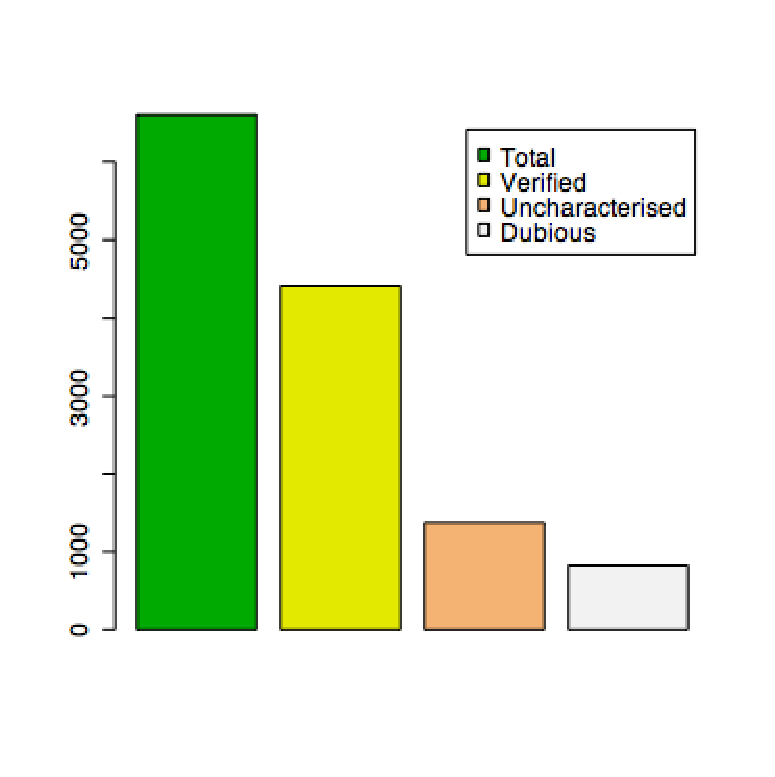
\includegraphics[scale=0.6]{sgd_orfs.eps}
\caption[ORF descriptions in the \emph{Saccharomyces} Genome Database]{Summary of ORF descriptions in the \emph{Saccharomyces} Genome Database, June 2006}
\label{figure:orf_totals}
\end{figure}

In \emph{S. cerevisiae}, as with other organisms, the field of functional genomics focuses on the identification and annotation of ORFs, the end goal being a complete map of all genes in the genome together with their role in cellular processes. Approaches to identifying genes often involve deleting the region of sequence thought to contain a gene, followed by identification of how the phenotype is affected; this method is aided by the simplicity with which specific sections of the yeast genome can be replaced via homologous recombination.

This technique, PCR-mediated targetted mutagenesis, relies on specific knowledge of the target region and the creation and insertion of a replacement cassette via PCR with a high degree of identity. This has the advantage that specific regions of sequence can be eliminated systematically, as well as the ability to completely remove the target gene which may not be the case using random insertional mutagenesis, described later. Furthermore, the incorporation of unique up and down tags for each mutant strain, as part of the insertion cassette, allows the amount of biomass of each mutant to be estimated by hybridisation of the extracted and PCR amplified tags using 5' prime radiolabelled nucleotides, this is outlined by Giaever \emph{et al.}\cite{Giaever1999} and in figure \vref{insertion_outline} of this report \cite{Delneri2004,Wach1996,Wach1994}.

\begin{figure}
\label{insertion_outline}
\centering
\includegraphics[scale=0.5]{insertion.eps}
\caption[Outline of PCR mediated mutagenesis]{Outline of PCR mediated mutagenesis protocol used to generate a hemizygous mutant in \emph{S. cerevisiae} taken from Giaver \emph{et al.} \cite{Giaever1999}. The parallel bars indicate the alleles on the two chromosomes. The lower allele has been replaced with the insertion cassette containing the kanamycin selection marker and unique molecular barcode. This tag can be amplified using the common primers as indicated in the diagram. The tag is hybridised to quantitatively estimate the amount mutant strain of which it identifies.}
\end{figure}

The benefits of using the ``molecular barcode'' strategy is that quantitative measurements can be produced for each gene deletion mutant, where even small changes in growth rate compared to wild type can be identified, as opposed to qualitative fitness descriptions which are statistically less useful \cite{Oliver2002,Winzeler1999}. This strategy was used by an international consortium in 2002 to characterise phenotype under six conditions for homozygous deletion mutants for 96\% the \emph{S. cerevisiae} annotated ORFs \cite{Giaever2002}. A paradigm for high-throughput functional genomics approaches this study determined which genes were essential to viability, as well as those that were non-essential but whose deletion resulted in a significantly slower growth rate.

Such large-scale studies, while providing large quantities of salient data, should not be considered a panopticon of gene and genome characterisation. Two \emph{in silico} studies of dispensability using genes involved in metabolism have shown that the essentiality of a gene depends both in what context the phenotype of the knockout is assessed as well as which other genes are present in the genome \cite{Pal2006,Papp2004}. Furthermore a study of ``silent'' mutations (genes whose deletion causes no discernible phenotype), showed that these deletions do have an effect on the concentrations of intracellular metabolites and that the role of the gene may be inferred from the levels of these metabolites within the cell \cite{Raamsdonk2001}. These instances have led to further studies where homozygous gene deletant strains were grown in several different media and gene functional assignments were made over a range of contexts; the goal being to make inferences of under which conditions a gene is essential \cite{Dudley2005,Giaever2002}.

Another method of value in functional genomics is insertional mutagenesis based on randomly mutating stretches of the \emph{S. cerevisiae} genome in an \emph{Escherichia coil} plasmid, followed by excision and insertion into the the genome via mitotic recombination \cite{Vidan2001}. This technique has the advantage that no prior knowledge of the target gene locations is required, and was usefully applied by Ross-Macdonald \emph{et al.} \cite{Ross-Macdonald1999} in identifying functional ORFs less than 50aa which had previously ignored due to the small size.

\subsubsection{Identifying gene function by partial suppression}

% Find out how many...
For certain genes under certain conditions deletion from the \emph{S. cerevisiae} genome results in an inviable mutant and therefore analysis of the homozygous deletant is not possible. This requires other strategies that allow the study of the role of the gene in cellular function; two techniques using the temporary or partial loss of gene function are the tetO-system and the construction of a hemizygous deletion mutant.

The tetO-system relies on the insertion of the \emph{tet} promoter upstream of the gene of interest. The activity of the genes under the control of the \emph{tet} promoter can be quantitatively controlled by the amount of doxycycline in the medium. The greater the quantities of doxycycline in the medium, the more the expression of the controlled gene is reduced. This allows the activity on the controlled genes to be precisely regulated by the concentration of doxycycline, and therefore the activity of the gene can be reduced without being completely removed \cite{Mnaimneh2004}.

The second strategy, the construction of a heterozygous deletion mutant, where only a single allele in a diploid strain is replaced with the null cassette, allows the analysis of the role of even essential genes, again based on reduced activity. Using the same method as for homozygous deletion mutants, it is possible to measure the heterozygous phenotypic effects quantitatively, using continuous culture and quantitative measurement of the molecular barcodes. Similarly to the homozygous mutant genome survey, heterozygous mutants were created for $\sim$5900 yeast ORFs and compared to wild-type growth in batch culture. Approximately 3\% of genes showed a reduced growth rate, half of these being annotated as being involved in metabolic processes \cite{Deutschbauer2005}. This figure however has been proposed to to be much higher 10\% - 12\%, when using a growth rate controlled continuous culture instead \cite{Papp2006}.

\subsection{Understanding gene function \emph{in silico}}

Determining the function of gene \emph{in silico} has the advantage over experimental approaches of being relatively faster and cheaper. Infering gene function through sequence similarity using BLAST \cite{blast} is widespread in molecular biology and the field of bioinformatics has developed genome wide comparisons \cite{blat} or more sensitive hidden markov model based searches \cite{hmmer}.

A systems biology approach to functional genomics will focus on the context of a gene in a dynamical system. In comparison to the described approaches for identification of essentiality \emph{in vivo}, a similar approach can be applied \emph{in silico} using flux balance analysis of genome scale metabolic models. Removal of a reaction in a genome scale model can be used to simulation the \emph{in vivo} process of gene knockout, as no flux can proceed through the reaction. When performed in the yeast genome scale model XXX \% of knockout phenotypes were correctly predicted. The advantage of using \emph{in silico} models is that even large scale functional genomic approaches can be performed easily. 

Genomic redundancy, where more than gene provides the same function, can be tested \emph{in vivo} through combined double deletion of gene pairs. In theory this would require ~6600$^2$ deleteion and be work intensive. Performin this \emph{in silico} is that this process would require only a little more time than the performing single deletions \emph{in silico}. Harrison \emph{et al.} \cite{double_deletion} showed that this approach can predict XXX \% of \emph{in vivo} double deletion phenotypes.

Genome scale models are well suited to the prediction of knockout phenotypes as there is a direct correspondence between the removal of a gene from the genome and the removal of the encoded enzyme in the metabolic network. When predicting phenotypes which are not simply a case of either on or off for the gene the analysis will be more complex. As an example gene dosage dependency can be analysed \emph{in vivo} through removal of one of the allelic copies of the gene. Performing this analysis with a genome scale model will be more complicated as the removal of half a gene does not translate so easily to the metabolic network. As example the removal of half a gene can be hypothesised not to result in a 50\% reduction in enzyme activity as transcription and translation of the gene may not follow linear dynamics, and even if this were the case enzyme kinetics often follow a non-linear response curve.

In addition to the above example of predicting haploid phenotypes, studying and predicting evolutionary effects in terms of the metablic network is also of interest. A substitution in the sequence of an enzyme encoding gene may have an effect on the corresponding kinetics of the encoded enzyme if the subsitution is in a region effecting the enzymes structure. The more important to growth, the greater the effect the mutation will have the competition of the organism in the environment. Therefore it may be possible to predict the selection pressure on the encoding gene based on the relevence to the phenotype of the organism. Similarly a mutational effect may not necessarily change the encoded protein sequence, but instead affect the rate at which the enzyme is translated through modification of the adaptation of the transcript for translation.

In Chapter 2 an approach was described using genome scale metabolic to estimate the control gene encoded reaction on the nutrient uptake fluxes of the organism. Using a subset of the reactions in the model that are encoded by a single gene, the relationship between the gene and the reaction is one to one. This should mean that any changes in the gene sequence should be directly reflected in the metabolic phenotype, this may not necessarily be the case if there were a homologue catalysing the same reaction. Therefore these gene cost measures can be tested to see if they reflect any the selection pressures described above. This may provide an indication if genome scale models and flux balance analysis are suitable techniques for making inferences about the evolution of gene sequence.

\subsection{Summary of results}

In this chapter the estimated gene costs from Chapter 2 are compared with a number of biological characteristics. First estimated gene cost is compared with data estimating the dosage dependency of yeast genes. Next the gene cost is compared with the estimated expression level of the gene. Finally gene cost is compared with evolutionary rate of the gene.

\section{Results}

\subsection{Gene sensitivity and haploinsufficiency}

\subsection{Gene sensitivity and expression}

\subsection{Gene sensitivity and evolutionary rate}

\section{Discussion}

\section{Materials and Methods}

\chapter{Discussion}
\input{5_discussion}

\bibliography{thesis}
\bibliographystyle{bmc_article}

\appendix
\addappheadtotoc
\appendixpage
\chapter{Amino Acids}
\include{6_amino_acids}

\end{document}
